\chapter{Introduction}

This is a book of drawings made in \LaTeX\  with Tikz\footnote{Pronounced "tics"} and other useful packages. Some drawings are in Portuguese.

%Dois pacotes ou comandos dão conflito. Package xypdf Error: pdfTeX version 1.40.0 or higher is needed for the xypdf. Já para usar o comando \begin{verbatim}\usegdlibrary{force}\end{verbatim} é preciso usar o Lua\LaTeX.

Although most drawings in this book of examples use Tikz\fnurl{https://ctan.org/pkg/pgf?lang=en}, there are some easier solutions for some specific drawings. Moreover, Tikz has multiple libraries that must be included, and I don't kept control of it, I just added everyone.

For example, chessboard\fnurl{https://ctan.org/pkg/chessboard?lang=en} is a useful package for drawing chess boards. I enjoy that it uses a very practical notation that is known to chess players.

The following code generates the image in \autoref{fig:chess}.


\begin{lstlisting}[style=myLateX,caption=Code for a Chess board]
\chessboard[addfen={bnrbnkrq/%
pppppppp/%
8/8/8/8/%
PPPPPPPP/BNRBNKRQ},showmover=false]
\end{lstlisting}

\begin{figure}
\centering
\chessboard[addfen={bnrbnkrq/%
pppppppp/%
8/8/8/8/%
PPPPPPPP/BNRBNKRQ},showmover=false]
\caption{A position form Fischer's Random Chess}
\label{fig:chess}
\end{figure}


\begin{figure}[hbt]
\centering
\begin{tikzpicture}[every node/.style = {minimum width=2cm,minimum height=1em,draw,font=\tiny,node distance=0cm,align=center}]
\node[fill=ibm1] (c1) at (0,0) {\#648fff};
\node[fill=ibm2,right = of c1] (c2)  {\#785ef0};
\node[fill=ibm3,right = of c2] (c3)  {\#dc267f};
\node[fill=ibm4,right = of c3] (c4)  {\#fe6100};
\node[fill=ibm5,right = of c4] (c5)  {\#ffb000};
\node[fill=black,text=white,right = of c5] (c6) {\#000000};
\node[fill=white,right = of c6] (c7) {\#ffffff};
\foreach \i in {100,95,...,0} {
\node[fill=ibm1!\i,below = of c1] (c1)  {};
\node[fill=ibm2!\i,right = of c1] (c21)  {};
\node[fill=ibm3!\i,right = of c21] (c31)  {};
\node[fill=ibm4!\i,right = of c31] (c41)  {};
\node[fill=ibm5!\i,right = of c41] (c51)  {};
\node[fill=black!\i,text=white,right = of c51] (c61) {} ;
\node[right = of c61] (c71) {$\i$\%} ;

};
\end{tikzpicture}
\caption{Cores da paleta sugerida pela IBM para daltonismo, com atenuação na cor para branco.}
\end{figure}



\begin{figure}[hbt]
\centering
\begin{tikzpicture}[every node/.style = {minimum width=2cm,minimum height=1em,draw,font=\tiny,,draw,node distance=0cm,align=center}]
\node[fill=ibm1] (c1) at (0,0) {\#648fff};
\node[fill=ibm2,right = of c1] (c2)  {\#785ef0};
\node[fill=ibm3,right = of c2] (c3)  {\#dc267f};
\node[fill=ibm4,right = of c3] (c4)  {\#fe6100};
\node[fill=ibm5,right = of c4] (c5)  {\#ffb000};
\node[fill=black,text=white,right = of c5] (c6) {\#000000};
\node[fill=white,right = of c6] (c7) {\#ffffff};
\foreach \i in {100,95,...,0} {
\node[fill=ibm1!\i!black,below = of c1] (c1)  {};
\node[fill=ibm2!\i!black,right = of c1] (c21)  {};
\node[fill=ibm3!\i!black,right = of c21] (c31)  {};
\node[fill=ibm4!\i!black,right = of c31] (c41)  {};
\node[fill=ibm5!\i!black,right = of c41] (c51)  {};
\node[fill=black,text=white,right = of c51] (c61) {$\i$\%} ;
\node[fill=white!\i!black,right = of c61] (c71) {} ;
};

\end{tikzpicture}
\caption{Cores da paleta sugerida pela IBM para daltonismo, com atenuação na cor para preto.}
\end{figure}


\begin{figure}[hbt]
\centering
\begin{verbatim}
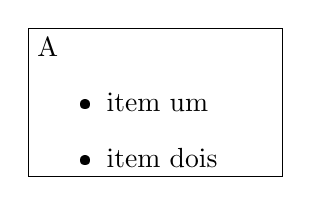
\begin{tikzpicture}
\node[draw,text width=3cm] at (0,0) {A
\begin{itemize}
    \item item um
    \item item dois
\end{itemize}
};
\end{tikzpicture}
\end{verbatim}
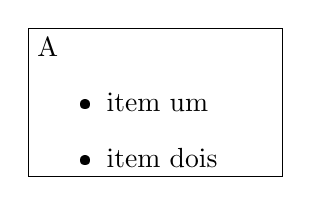
\begin{tikzpicture}
\node[draw,text width=3cm] at (0,0) {A
\begin{itemize}
    \item item um
    \item item dois
\end{itemize}
};
\end{tikzpicture}
\caption{Itemize no nó precisa transformar o nó de mbox para minipage, e o text width faz isso. \url{https://tex.stackexchange.com/questions/213662/enumerate-within-tikz-node}}
\end{figure}